\documentclass[a4paper, 14pt]{extarticle}

% Useful packages
\usepackage{amsmath, amsfonts, amssymb} % AMS math packages
\usepackage{caption} % for custom captions
\usepackage{minted} % for code highlighting
\usepackage{fancyvrb} % For enhanced verbatim features
\usepackage{graphicx} % For including graphics
\graphicspath{{figures/}}
\usepackage{siunitx} % For typesetting SI units
\usepackage[colorlinks=true, allcolors=black]{hyperref} % Hyperlinks with black color
\usepackage{listings} % for code formatting
\usepackage{xcolor} % for color
\usepackage{multirow}
\usepackage{multicol}
\usepackage{adjustbox}
\usepackage{booktabs}
\usepackage{grffile} % Improved file name support for graphics
\usepackage{subcaption} % Subfigure and subcaption support
\usepackage{float} % Improved float placement
\usepackage{setspace} % Set space between lines
\usepackage[11pt]{extsizes} % Extends document class options
\usepackage[numbers]{natbib} % For numeric citations
\usepackage{changepage} % Added for adjustwidth environment
\usepackage[a4paper,top=3cm,bottom=1.5cm,left=2cm,right=2cm]{geometry}
\usepackage{pdfpages}

\usepackage{fancyhdr} % Customizing headers and footers
\setlength{\headheight}{0pt} % Setting the height of the header
\addtolength{\topmargin}{0.2cm} % Adjusting the top margin

\usepackage{titletoc} % Customizing table of contents
% Define the page style
\fancypagestyle{customstyle}{
  \fancyhf{} % Clear header and footer
  \fancyhead[L]{Team 494, Problem A} % Left header
  \fancyhead[R]{Page \thepage\ out of 24} % Right header with page number
  \renewcommand{\headrulewidth}{0.4pt} % Horizontal line under the header
}
% Apply the custom page style
\pagestyle{customstyle}

% To include pdf : \includepdf[pages=-, angle=270]{A1-graph.pdf}

% Define custom colors
\definecolor{commentgreen}{rgb}{0,0.5,0}
\definecolor{keywordblue}{rgb}{0,0,0.8}
\definecolor{stringred}{rgb}{0.8,0,0}

% Configure listings for Python
\lstset{
    language=Python,
    basicstyle=\ttfamily\small, % font size
    keywordstyle=\color{keywordblue}\bfseries, % keywords in blue and bold
    commentstyle=\color{commentgreen}, % comments in green
    stringstyle=\color{stringred}, % strings in red
    numbers=left, % line numbers on the left
    numberstyle=\tiny\color{gray}, % line numbers style
    stepnumber=1, % line numbers step
    frame=single, % adds a frame around the code
    tabsize=4, % tab space width
    showstringspaces=false, % don't show spaces in strings
    captionpos=b, % caption position
    breaklines=true, % wrap long lines
    breakatwhitespace=false,
    escapeinside={(*@}{@*)} % if you need LaTeX inside code
}
%-------------------------------
% Document begins
%-------------------------------
\begin{document}
% Front page content
% \vspace{-9cm}
\title{Micrometeorite Threats: An analysis for the air pressure loss due to meteorite-induced puncture in space stations by modeling depressurization dynamics.}
\author{\textbf{Problem A:} Space Station Air Evacuation Time\\Team 494}
\date{November 4, 2024}
\maketitle
%___________________________________________________________%
\begin{abstract}
\normalsize % Options include \large, \Large, \LARGE, etc.
Micrometeorites and space debris continuously crashes onto spacecrafts which can potentially puncture the spacecrafts.
This study examines the depressurization dynamics of a space station following a micrometeorite puncture. The model uses a cylindrical space station with a volume of approximately 628 $m^3$, an initial air pressure of 1 $atm$ and a temperature of $\SI{20}{\degreeCelsius}$. A 1 $cm$-diameter orifice allows air to escape into the vacuum of space, while the depressurization is approximated as an adiabatic process. Using a discharge coefficient of 0.6, we estimate the mass flow rate through the hole, followed by continuous pressure, temperature, and density change as the air escapes. Our findings indicate that the internal pressure reaches 30\% of the initial pressure i.e, 0.3 $atm$ ($\approx30.39\,kPa$) in about 10 $hr$ for a 1 $cm$ hole. In contrast, for a 5 $cm$-diameter puncture, the time drastically decreases to just 24 $min$. This study highlights that small punctures do not result in immediate loss of life-supporting pressure and provide valuable response time, whereas, a larger orifice significantly reduce the response time, increasing hazard levels. These results emphasize the need for effective leak detection and rapid repair protocols to enhance astronaut safety during micrometeorite impacts.

\textbf{Keywords:} Spacecraft depressurization, micrometeorite impact, mass flow rate, pressure drop dynamics, choked flow, Knudsen number, quasi-static adiabatic process.
\end{abstract}
\newpage
%___________________________________________________________%
\tableofcontents
\newpage
\section{Introduction}
%___________________________________________________________%
\subsection{Historical Background}
On the night of 29 August, 2018, a small air leak on the Soyuz MS-09, a spacecraft that transported three members of the Expedition 56/57 crew to the international space station (ISS), was noticed by the ground control. A 2 $mm$ hole on this spacecraft was discovered that caused the station to start depressurizing at a slow rate. Before the crew members solved it with epoxy sealent, European Space Agency (ESA) astronaut \textit{Alexander Gerst} reportedly put his finger over the hole to try to plug the leak. \citep{guardian2018issleak} \citep{dailymail2018issleak}

%___________________________________________________________%
\begin{figure}[ht]
  \begin{subfigure}{0.5\textwidth}
    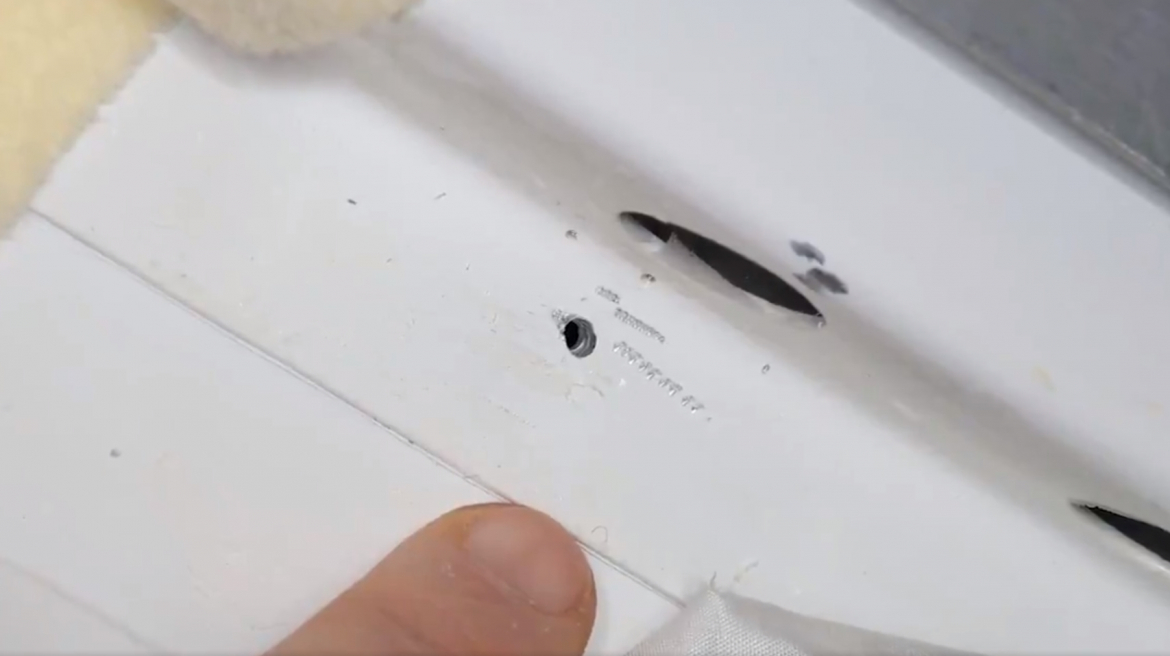
\includegraphics[width=0.9\linewidth, height=4cm]{before_leak}
    \caption{Before sealing}
  \end{subfigure}
  \hfill
  \begin{subfigure}{0.55\textwidth}
    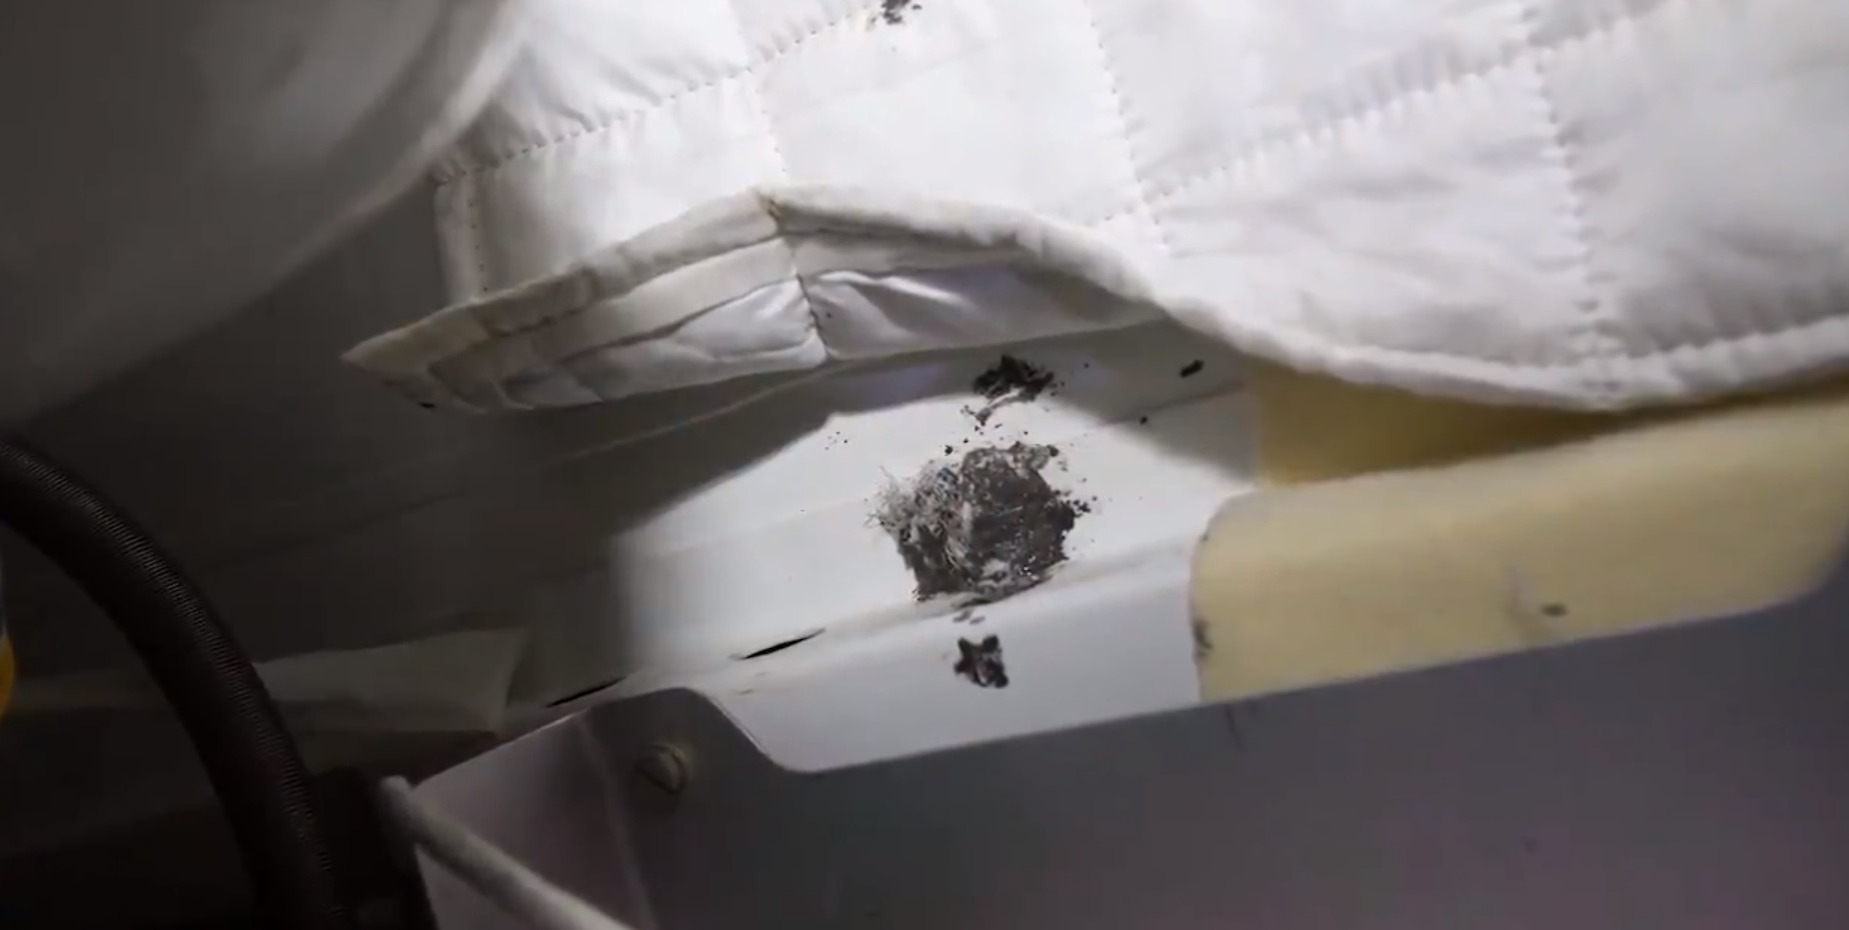
\includegraphics[width=0.85\linewidth, height=4cm]{after_leak}
    \caption{After sealing}
  \end{subfigure}
  \caption{A small air leak on the Soyuz MS-09, 29 August, 2018 \citep{nasaspaceflight2018issleak} }
\end{figure}

Similar incidents happened with Gaia \citep{esa2024} and the James Webb Space Telescope (JWST) \citep{jwst2022} where a meteorite hit may have caused significant damage.

This kind of meteorite or space debris collision poses a potential threat to the spacecraft and humans inside it. Meteorite can travel as fast as 12-40 $km\,s^{-1}$ \citep{wustl2024} and space debris can reach upto speed of $8\, km\,s^{-1}$ \citep{nasa2024}. A collision with meteorite or space debris at these high speeds can cause major damage to any spacecraft. Thus it is crucial to assess the outcome and threats of these incidents. In this paper we will evaluate the effect on pressure inside the spacecraft caused by a hole created through a micrometeorite, which is a major factor for survival of the spacecraft and the humans inside it.
%___________________________________________________________%
\subsection{Problem restatement}
We have an approximately cylindrical space station which has a diameter and length of $4\, m$ and $50\, m$ respectively. The air inside the space station is at a temperature of $\SI{20}{\degreeCelsius}$ and a pressure of 1 atm (101.3 $kPa$). A hole of 1 $cm$ in diameter is created from an impact of a micrometeorite at the center of one end of the space station. As the air inside escapes or flows out through this hole, the pressure of the air inside starts to decrease. Here our primary task is to determine the time needed for the air pressure inside the space station to drop from 1 $atm$ to 0.3 $atm$.

After we estimate the depressurization time for this hole, we need to evaluate how the holes having different diameter will have effect on this depressurization time i.e, we have to analyze and establish a relation between the depressurization time and the diameter of the hole caused by the micrometeorite impact on the space station.

%___________________________________________________________%

\section{Notations}
\begin{table}[H]
\centering
\def\arraystretch{1.4}
\begin{tabular}{lp{3in}c}
\hline
Symbols & Explanations & Numerical Value \\ \hline
$k_B$ & Boltzmann constant & $1.38 \times 10^{-23}\,J\,K^{-1}$ \\
$N_A$ & Avogadro constant & $6.02214076\times 10^{23}\,mol^{-1}$ \\
$\gamma$ & Specific heat ratio for air & $1.4$ \\
$\mathcal{R}$ & Universal gas constant & $8.314 \, J/(mol \cdot K)$ \\
$R$ & Specific gas constant for air & $287.12 \, J/(kg \cdot K)$ \\
$M_a$ & The molecular weight of air & $28.96\times 10^{-3} \, kg/mol$ \\
$\mathcal{K}$ & Adiabatic constant & $28.27$ \\
$n$ & Number of moles & \\
$\mathcal{D}$ & Diameter of a gas molecule & \\
$\dot{m}$ & The mass flow rate & \\
$A$ & Area of the orifice & \\
$P_t$ & Stagnation (or total) pressure & \\
$T_t$ & Stagnation (or total) temperature &  \\
$P_i$ & Initial pressure & $101.3\times 10^3 \, Pa$ \\
$T_i$ & Initial temperature & $\SI{20}{\degreeCelsius}=293\,K$  \\
$P$ & Static pressure & \\
$V$ & Spacecraft volume & 628.32 $m^3$ \\
$T$ & Static temperature &  \\
\hline
\end{tabular}
\end{table}
%___________________________________________________________%
\section{Assumptions}
\subsection{Composition of the air inside the space station}
The composition of the air inside the space station is assumed to be similar to the atmosphere of Earth. This is because in the real case scenario, we can consider the composition of air inside the ISS which is kept similar to Earth's atmosphere (79\% $N_2$ and 21\% $O_2$) to maintain Earth like environment inside the space station \citep{wiki2024}.

\subsection{Model of the air inside the space station}
The air inside is also assumed to act as an ideal gas since the volume of the space station is way larger than the combined volume of the air molecules inside it. This assumption is also reasonable since the pressure and temperature inside the space station is similar to the typical pressures and temperatures found in Earth at ground level. This allows us to apply the ideal gas law, 
\[ PV \,=\, n\mathcal{R}T \]

\subsection{Nature of the depressurization process}
The depressurization process of the air is assumed to be adiabatic in nature. This assumption is based on the fact that for a rapid depressurization event, usually there isn’t enough time for significant heat to be transferred between the gas inside the station and the surrounding walls or the external environment.

\subsection{Outside pressure}
The outside pressure due to the escaped gas is assumed to be nearly zero. This is because the atmospheric pressure at an altitude of 400 $km$ (which is the altitude of ISS) is around $1.5 \times 10^{-9}\, kPa$ \citep{usgovt}, which can be approximated as zero when we deal with atmospheric pressures. Additionally, there is no finite space or a container for the gas molecule that is escaped through the hole can have any impact. Thus we can assume that any development of external pressure due to the escaped gas is very unlikely, as the escaped gas molecules will spread throughout the infinite space and lost forever.
%___________________________________________________________%

\section{Establishment of the model}
Our goal is to estimate the time that is required for the air pressure inside the space station to fall from an initial value of 1 $atm$ to a final value of 0.3 $atm$. With the assumptions in consideration, we now begin to establish a mathematical model to reach our goal.

\subsection{Continuum Hypothesis}
As we begin to establish the model, we ask the question if we can treat the flow of air as a continuum flow. It is necessary because the laws of fluid mechanics hold true only when we can consider a fluid as a continuous media.

The continuum hypothesis is valid when the mean free path of molecules i.e., the average distance a molecule travels between collisions, is much smaller than the characteristic length scale of the flow i.e., the diameter of the hole in our case. This condition can be represented using the \textit{Knudsen Number}, which is defined as,
$$K_n = \frac{\lambda}{L}$$
Depending on the value of the Knudsen number, the flow of a fluid is classified into four main categories:
\begin{enumerate}
    \item \textbf{Continuum Flow ($K_n < 0.001$):}  In this regime, the mean free path of the molecules is much smaller than the characteristic length scale of the flow. Fluid properties can be described continuously.
    \item \textbf{Slip Flow} ($0.001 < K_n <0.1$): In this regime, the mean free path is still small compared to the characteristic length, but slip at boundaries is non-negligible.
    \item \textbf{Transitional Flow ($0.1 < K_n < 10$):} In this regime, The flow exhibits a mix of continuum and free molecular flow characteristics. Molecular interactions are significant throughout the flow, but some continuum mechanics may still apply.
    \item \textbf{Free Molecular Flow $(K_n > 10)$:} In this regime, the mean free path is much larger than the characteristic length; in this regime, the laws of fluid mechanics which assume fluids to be continuous media, fail to hold \citep{bird1994}.
\end{enumerate}
\begin{figure}[H]
\centering
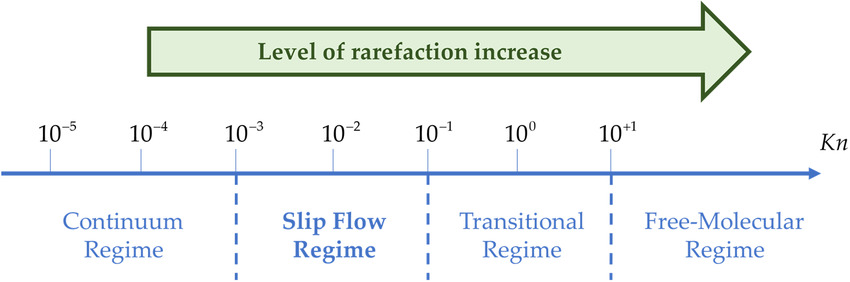
\includegraphics[width=0.9\linewidth]{knudsen_number.jpg}
\caption{Flow classification depending on the Knudsen number}
\end{figure}
\subsubsection*{Determining the Knudsen number, $K_n$}
From the kinetic theory, the mean free path $\lambda$ is given by:
\[ \lambda = \frac{k_B T}{\sqrt{2} \pi \mathcal{D}^2 P} \]
The molecular diameter $\mathcal{D}$, i.e., the diameter of a gas molecule can be determined through the Van der Waals constant $b$, that is related to the effective volume occupied by gas molecules and given by \citep{atkins2006},
\begin{align*}
    b &= \frac{16 \pi \mathcal{D}^3}{3} \times N_A \\
    \therefore \mathcal{D} &= \left( \frac{3b}{16 \pi N_A} \right)^{1/3}
\end{align*}
From the composition of air, (78\% $N_2$, 21\% $O_2$), $b_{air}$ is approximated as,
\[ b_{air} \approx 0.037 \, L\,mol^{-1} = 0.037 \times 10^{-3} \,m^3\,mol^{-1} \]
Putting the values we get, 
$$\mathcal{D} = 1.542 \times 10^{-10} \,m$$
The mean free path for the air inside the space station is then,
$$\therefore \lambda = \frac{k_B T}{\sqrt{2} \pi \mathcal{D}^2 P} = 0.000379 \,cm$$
Finally we get the Knudsen number $K_n$,
$$\therefore K_n = \frac{\lambda}{L} = \frac{0.000379\,cm}{1\,cm} = 0.000379 < 0.001 $$
Therefore, the flow of the air in our case can be treated as continuum flow.

\subsection{Determination of the type of flow on the basis of pressure}
When a compressible fluid (in this case, air) flows through a restriction (eg. orifice, nozzle, valve, etc.) due to the difference between upstream and downstream pressure, two types of situation can occur depending on the ratio of downstream pressure ($P_d$) and upstream pressure ($P_u$) :
\begin{itemize}
    \item [(i)] \textbf{Non-Choked Flow:} This occurs if the pressure ratio satisfies
    \begin{align*}
        \left(\frac{\gamma+1}{2}\right)^{-\gamma/(\gamma-1)} &\leq \frac{P_d}{P_u} \leq 1 \\
        \Rightarrow 0.528 &\leq \frac{P_d}{P_u} \leq 1
    \end{align*}
    In this situation, the fluid velocity increases as downstream pressure \(P_d\) decreases or upstream pressure \(P_u\) increases.
    
    \item [(ii)] \textbf{Choked Flow:} This occurs if 
    \begin{align*}
        \frac{P_d}{P_u} &\leq \left(\frac{\gamma+1}{2}\right)^{-\gamma/(\gamma-1)} \\
        \Rightarrow \frac{P_d}{P_u} &\leq 0.528
    \end{align*}
    Here, the fluid velocity reaches the speed of sound. Increasing \(P_u\) does not further raise fluid velocity, though the mass flow rate still depends on upstream pressure, temperature, and orifice area.
\end{itemize} 
In our problem, since we assumed that the downstream pressure i.e. the outside pressure of the space station will remain nearly zero throughout the process, the ratio $\frac{P_d}{P_u}$ will approach zero. Therefore, according to the conditions, we conclude that the flow of air will be choked \citep{anderson}.
%___________________________________________________________%
\subsection{Expression for the mass flow rate}
So far we have seen that the flow of the gas through the hole can be treated as continuous flow thus the laws of  fluid mechanics will be obeyed. Additionally taking into consideration that the nature of the flow is adiabatic, we can employ the expression for the mass flow rate for an isentropic flow since in an adiabatic process the entropy stays the same.\\ \\
For an ideal compressible gas, the mass flow rate equation is given\citep{nasa_cal}\citep{albright2010}:
$$ \dot{m} = C_d\,A\, \frac{P_t}{\sqrt{T_t}} \sqrt{\frac{\gamma}{R}} \, M \left( 1 + \frac{\gamma - 1}{2} M^2 \right)^{-\frac{\gamma + 1}{2(\gamma - 1)}} $$
For choked flow we have $M = 1$, thus,  the mass flow rate simplifies into:
\begin{align*}
    \dot{m} = \frac{C_dA P_t}{\sqrt{T_t}} \sqrt{\frac{\gamma}{R} \left( \frac{2}{\gamma + 1} \right)^{\frac{\gamma + 1}{\gamma - 1}}}
\end{align*}
Substituting the values for air, we get:
\begin{align}
    \dot{m} = 0.0404 \times \frac{C_dA P_t}{\sqrt{T_t}}
\end{align}
The stagnation properties are related to the static properties by:
\begin{align*}
    P_t &= P \left( 1 + \frac{\gamma - 1}{2} M^2 \right)^{\frac{\gamma}{\gamma - 1}} \\
    T_t &= T \left( 1 + \frac{\gamma - 1}{2} M^2 \right)
\end{align*}
Substituting the values for air at choked conditions where \( M = 1 \), we get:
\begin{align*}
    P_t &= 1.892929 \times P \\
    T_t &= 1.2 \times T
\end{align*}
The mass flow rate in equation (1) simplifies to:
\begin{align*}
    \dot{m} &= 0.0404\times \frac{C_d A\cdot (1.892929 \times P) }{\sqrt{(1.2 \times T)}}
\end{align*}
\begin{align}
    \therefore \dot{m} &= 0.06985\times \frac{C_d A\,P}{\sqrt{T}}
\end{align}

\subsection{Expression for the pressure and temperature}
For an adiabatic process, we have:
\begin{align}
    P^{1 - \gamma} T^{\gamma} = \text{constant} = \mathcal{K}
\end{align}
We find $\mathcal{K}$ from the initial condition,
\[
\mathcal{K} = P_i^{1 - \gamma} T_i^{\gamma} \approx 28.27
\]
Now, we know from the ideal gas law,
\begin{align*}
    PV &= n\mathcal{R} T \\
    \Rightarrow PV &= \frac{m}{M_a} \mathcal{R} T \\
    \Rightarrow P &= \left(\frac{m}{V}\right) \left(\frac{\mathcal{R}}{M_a}\right) T \\
    \therefore P &= \rho R T \\
    \therefore T &= \frac{P}{\rho R}
\end{align*}
Substituting this temperature in equation (3) we get,
\begin{align*}
    P^{1 - \gamma} \left( \frac{P}{\rho R} \right)^{\gamma} &= \mathcal{K} \\
    \Rightarrow P^{1 - \gamma + \gamma} \left( \frac{1}{\rho R} \right)^{\gamma} &= \mathcal{K} \\
    \therefore P = \mathcal{K} \times (\rho R)^{\gamma}
\end{align*}
Substituting the temperature we get,
\begin{align*}
    \therefore T &= \frac{P}{\rho R} \\
    \Rightarrow T &= \frac{\mathcal{K} \times (\rho R)^{\gamma}}{\rho R} \\
    \therefore T &= \mathcal{K} \times (\rho R)^{\gamma-1} \\
\end{align*}

\subsection{Variation of the pressure and temperature as function of time}
\vspace{1cm}
In this section, we utilize a computational approach to evaluate pressure and temperature as functions of time. The process begins with initial values of pressure ($P_i=101.3\,kPa$) and temperature ($T_i=293\,K$) to determine the initial mass flow rate $\dot{m}$ using the derived relation in equation (2).
\newpage
Next, we calculate the amount of air that escapes from the station over a small time interval $dt$. This value is then used to assess the change in net mass within the station during that interval, which allows us to update the air density inside the station. \\

Using this updated density, we proceed to calculate the new values for pressure and temperature. These updated parameters then enable us to compute a new mass flow rate after the elapsed time $dt$. This iterative algorithm continues to update the pressure and temperature, providing a time-dependent view of these variables. The resulting variations of pressure and temperature are presented in graphs (as illustrated in Appendix A). 
\begin{figure}[H]
\centering
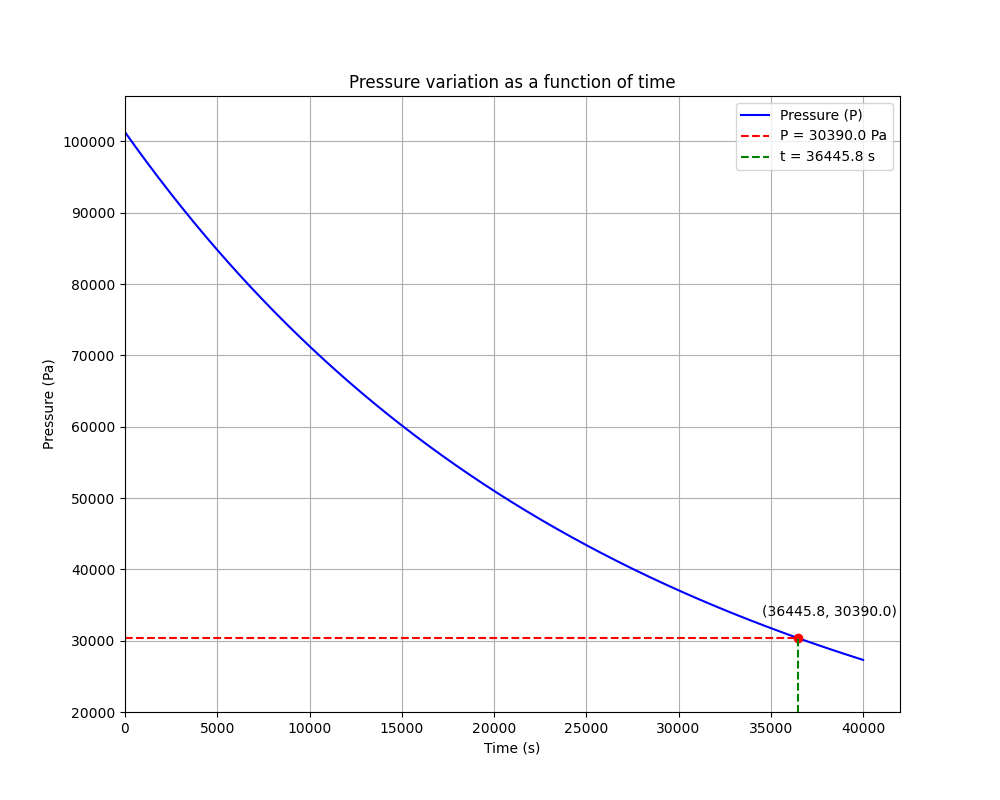
\includegraphics[width=1\linewidth]{pressure_plot.png}
\caption{Variation of pressure as a function of time}
\end{figure}
\begin{figure}[H]
\centering
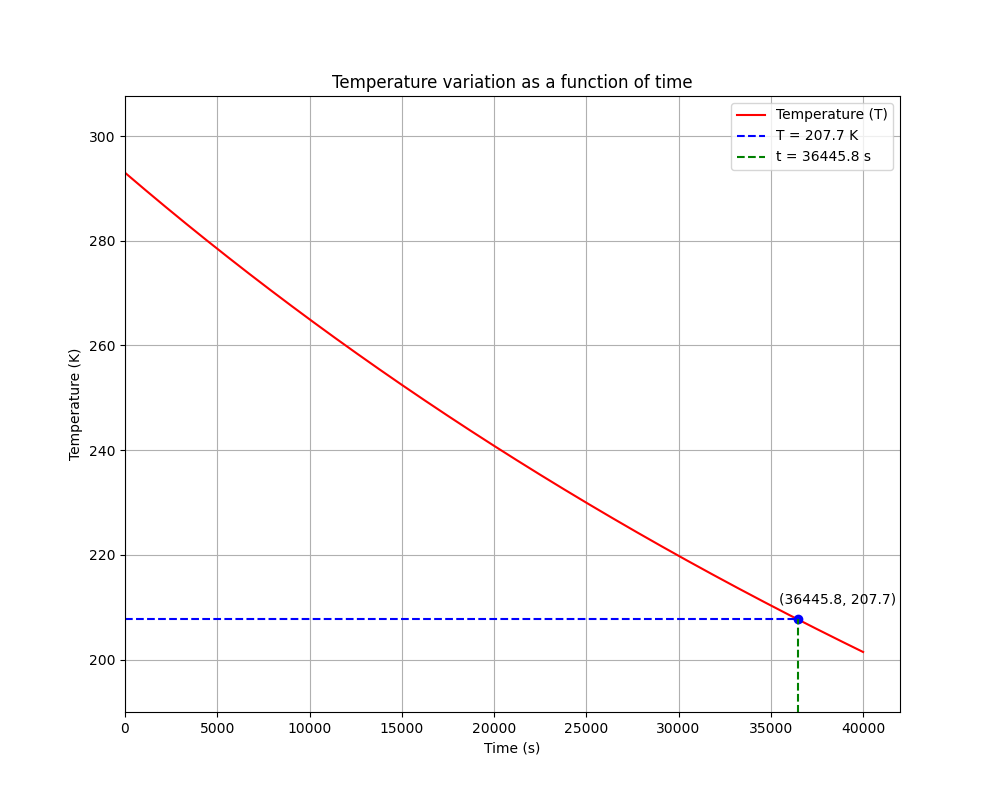
\includegraphics[width=1\linewidth]{temperature_plot.png}
\caption{Variation of temperature as a function of time}
\end{figure}

From the analysis in Appendix B, we can determine the total time required for the pressure in the station to decrease from 1 $atm$ (101.3 $kPa$) to 0.3 $atm$ (30.39 $kPa$) through a hole with a diameter of 1 $cm$. This time is approximately 36500 $sec = \left(\frac{36500}{3600}\right) \approx 10.13 \,hours$
\newpage
\subsection{Effect of the hole diameter on the required time}
The code given in the Appendix C gives us the variation of required time with respect to the hole diameter
\begin{figure}[H]
\centering
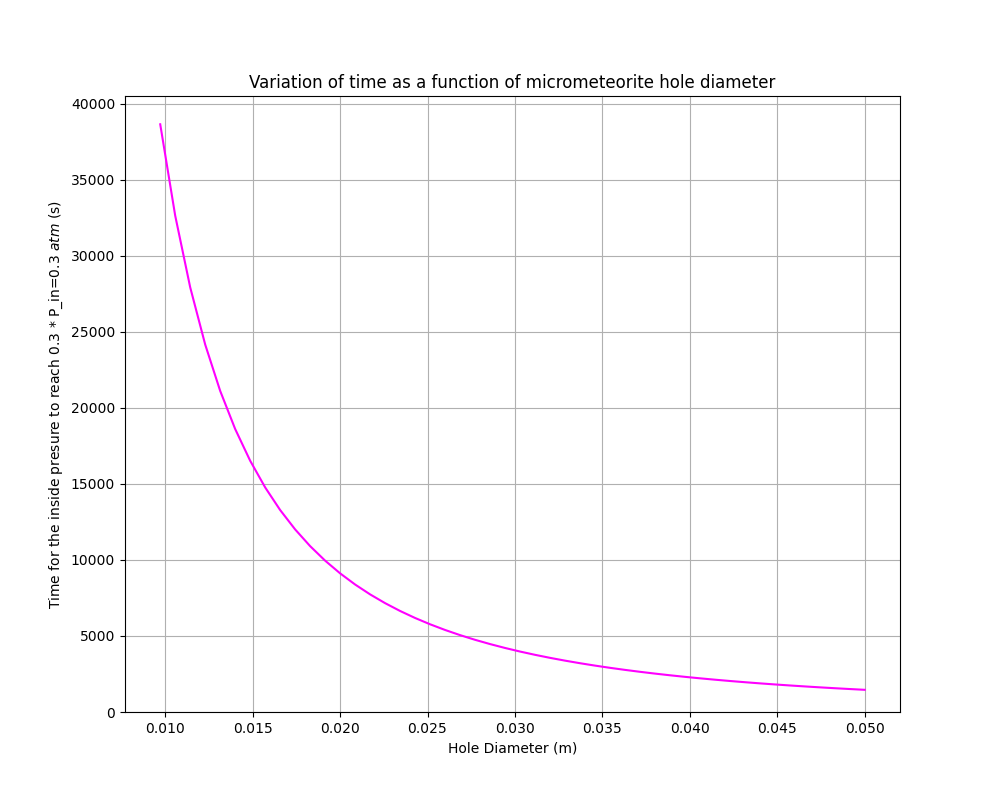
\includegraphics[width=0.9\linewidth]{diameter_plot.png}
\caption{Variation of time as a function of hole diameter}
\end{figure}
To compare the required time for a orifice 1 $cm$ in diameter with the required time for a larger orifice, we evaluated the required time for a orifice 5 $cm$ in diameter, which came out to be around 24 $minutes$.

\section{Result}
The time required for the internal pressure of the space station to decrease from an initial value of 101.3 $kPa$ to a target pressure of 30.39 $kPa$ (0.3 $atm$) was calculated using a computational model assuming choked flow conditions through a puncture in the station. The geometry of the space station was modeled as a cylinder with a radius of 2 $m$ and a length of 50 $m$. A hole with a radius of 0.5 $cm$ was considered for this analysis, resulting in a calculated depressurization time of approximately 10 $hours$.
Further analysis revealed a significant relationship between the diameter of the hole and the time required for the pressure to reach the target level. Specifically, as the diameter of the puncture increased, the time for the pressure to drop to 0.3 atm decreased substantially. This indicates that larger breaches lead to more rapid depressurization, primarily due to the increased mass flow rate of air escaping the chamber. The implications of these findings suggest that even small enhancements in the diameter of a puncture can critically affect the structural integrity and safety protocols of space habitats.

\section{Result evaluation}
The analysis indicates that depressurization due to a small puncture in a space station—such as a hole with a radius of 0.5 $cm$—does not lead to an immediate, life-threatening drop in pressure for the inhabitants. Given the estimated time of approximately 10 $hr$ to reach a critical low pressure of 0.3 $atm$, the gradual nature of the pressure loss suggests that prompt action can mitigate significant risk. If a small puncture is identified and repaired within an hour, the station's atmosphere remains sufficiently stable to ensure the safety of its occupants. This was evidenced by the incident on Soyuz MS-09, where after a small hole was detected, an astronaut managed to temporarily seal it with a finger, and a more durable repair was made with epoxy sealant shortly thereafter.

\section{Model Evaluation}
\subsection{Strengths}
\subsubsection*{Straightforward Model}
Our model is straightforward and easy to analyze, using equations that are simple to understand and implement.
\subsubsection*{Quick estimation}
The model provided a quick and effective estimate of the time required for the pressure to drop to a specified level, allowing for timely assessment of depressurization risks in emergency situations.
\subsubsection*{Accessibility}
Our model is built on fundamental principles of physics, making it accessible and understandable to a broad audience. 

\subsection{Weaknesses}
\subsubsection*{Approximation of Discharge Coefficient}
In our model, we used an approximate discharge coefficient ($C_d$) value of 0.6 to estimate the flow rate through the orifice. While this value is a reasonable approximation, $C_d$ can vary depending on factors like orifice geometry, fluid properties, and flow conditions. Using a constant $C_d$ introduces some approximation error, as an exact value would require a more detailed analysis or experimental data. However, this approximation provides a practical estimate within an acceptable range for this type of application.
\subsubsection*{No heat transfer effect}
While the adiabatic assumption simplifies calculations, it may not fully capture thermal effects if depressurization occurs over extended periods, during which heat exchange could influence pressure and temperature.
\subsubsection*{Ideal gas consideration}
We assumed the gas to obey the ideal gas laws. It may have caused slight inaccuracy, which can be mitigated by considering the equations for real gas.
%___________________________________________________________%
\section{Conclusion}
This analysis emphasizes the importance of structural integrity around potential breach points; despite the rapid outflow of air due to sonic conditions, the rate of depressurization remains controlled enough to allow for intervention. The relatively slow depressurization also underscores the robustness of space station habitats, which are engineered to withstand small punctures without catastrophic failure. Moreover, this scenario suggests that real-time detection and response protocols, along with effective sealing materials, play a crucial role in ensuring crew safety in the event of a puncture.
In evaluating this result, it becomes clear that while small punctures may not pose an immediate threat, larger breaches would significantly accelerate pressure loss, potentially reaching dangerous levels more quickly. Thus, this study underlines the importance of regular structural assessments, detection systems for breaches, and ready access to repair materials on space stations, providing critical insights for the design and operation of safe, resilient human habitats in space.

% References------------------------------------------------
% Add the bibliography section with numbered references
\addcontentsline{toc}{section}{References}
\bibliographystyle{unsrtnat}
\bibliography{494A-references}
% \addcontentsline{toc}{section}{References}
% \bibliographystyle{unsrtnat}  % Specify the bibliography style (unsrtnat for numbered references)
% \bibliography{guardian, dailymail, nasa_leak, esa2024, jwst2022, wust, nasa2024, wiki2024, usgovt, atkins2006, bird1994, anderson, nasa_cal, alb}  % Specify the names of your .bib files, separated by commas
\newpage
%___________________________________________________________%
\section*{Appendices}
\addcontentsline{toc}{section}{Appendices}
\textit{\textbf{Python source codes}}
\subsection*{A}
\begin{lstlisting}[language=Python]
import numpy as np
import matplotlib.pyplot as plt

# Cylinder volume & nozzle area
L = 50                      # Length of cylinder in meters
R = 2                       # Radius of cylinder in meters
V = np.pi * R ** 2 * L      # Volume of the cylinder, in m^3
d = 1E-2                    # Diameter of the nozzle in meters
A = np.pi * (d/2) ** 2      # Cross-sectional area of the nozzle, in m^2

# Gas constants 
Y = 1.4                     # Specific heat ratio
R_gas = 287.12                 # Specific gas constant for air in J/(kg*K)

# Initial conditions
P_i = 101.3e3               # Initial pressure in Pa
T_i = 273 + 20              # Initial temperature in K
rho_i = P_i / (R_gas * T_i) # Initial density, in kg/m^3
m_i = rho_i * V             # Initial mass, in kg

# Initial variables
m = m_i
P = P_i
T = T_i
k = P_i**(1 - Y) * T_i**Y   # constant for calculations

# Define the function
def rho(m_in):
   return m_in/V

# Time step and data lists
dt = 0.1
P_data = []
T_data = []
t_data = []

# Simulation loop
for t in np.arange(0, 40000, dt):
    P_data.append(P)
    T_data.append(T)
    t_data.append(t)

    # Calculate mass flow rate
    m_dot = 0.6 * 0.06985 * A * (P / np.sqrt(T))
    m = m - m_dot * dt

    # Update pressure and temperature
    P = k * (rho(m) * R_gas)**Y
    T = k * (rho(m) * R_gas)**(Y - 1)

# Define target pressure and find intersection time
target_pressure = 0.3 * P_i  # 30% of initial pressure
intersection_time = None

# Find the time at which pressure reaches target_pressure
for i, pressure in enumerate(P_data):
    if pressure <= target_pressure:
        intersection_time = t_data[i]
        break
    
# First plot: Pressure vs Time with limited horizontal and vertical lines, with time axis starting from zero
plt.figure(figsize=(10, 8))
plt.plot(t_data, P_data, color='blue', label='Pressure (P)')
plt.plot(intersection_time, target_pressure, 'ro')  # Mark intersection point

# Horizontal and vertical lines from axes to intersection point only
plt.hlines(y=target_pressure, xmin=0, xmax=intersection_time, color='red', linestyle='--', label=f'P = {target_pressure:.1f} Pa')
plt.vlines(x=intersection_time, ymin=0, ymax=target_pressure, color='green', linestyle='--', label=f't = {intersection_time:.1f} s')

# Adding coordinates at the intersection point
plt.text(intersection_time - 2000, target_pressure + 3000, f'({intersection_time:.1f}, {target_pressure:.1f})', color='black')
plt.xlabel('Time (s)')
plt.ylabel('Pressure (Pa)')
plt.title('Pressure variation as a function of time')
plt.xlim(left=0)  # Ensure time starts from zero
plt.ylim(bottom=20000)
plt.grid(True)
plt.legend()
plt.savefig("pressure_plot.png", format="png")
plt.show()

# Second plot: Temperature vs Time with lines from intersection point to axes, and time axis starting from zero
plt.figure(figsize=(10, 8))
plt.plot(t_data, T_data, color='red', label='Temperature (T)')
plt.plot(intersection_time, T_data[t_data.index(intersection_time)], 'bo')  # Mark intersection point

# Horizontal and vertical lines from axes to intersection point only
plt.hlines(y=T_data[t_data.index(intersection_time)], xmin=0, xmax=intersection_time, color='blue', linestyle='--', label=f'T = {T_data[t_data.index(intersection_time)]:.1f} K')
plt.vlines(x=intersection_time, ymin=0, ymax=T_data[t_data.index(intersection_time)], color='green', linestyle='--', label=f't = {intersection_time:.1f} s')

# Adding coordinates at the intersection point
plt.text(intersection_time - 1000, T_data[t_data.index(intersection_time)] + 3, f'({intersection_time:.1f}, {T_data[t_data.index(intersection_time)]:.1f})', color='black')
plt.xlabel('Time (s)')
plt.ylabel('Temperature (K)')
plt.title('Temperature variation as a function of time')
plt.xlim(left=0)
plt.ylim(bottom=190)
plt.grid(True)
plt.legend()
plt.savefig("temperature_plot.png", format="png")
plt.show()
\end{lstlisting}
\newpage
\subsection*{B}
\begin{lstlisting}[language=Python]
import numpy as np

# Constants
Y = 1.4
R = 2                   # Radius in meters
L = 50                  # Length in meters
V = np.pi * R ** 2 * L  # V of the space station

r = 0.5E-2              # Hole radius in meters
A = np.pi * r ** 2      # Area of the hole

# Gas constants and initial conditions
R_GAS = 287.12          # Specific gas constant for air (J/kg K)
P_i = 101.3e3           # Initial pressure in Pa
T_i = 273 + 20          # Initial temperature in K
rho_i=P_i/(R_GAS*T_i)   # Initial density

m_i = rho_i * V         # Initial mass of air in the station

# Initial state
mass = m_i
pressure = P_i
temperature = T_i
k = P_i**(1-Y)*T_i** Y  # Adiabatic constant

# Target pressure (30% of the initial pressure)
TARGET_PRESSURE = 0.3 * P_i
dt = 0.1                # Time step in seconds

# Variable to store the time when pressure reaches the target
time_to_reach_target = None
target_pressure_reached = False
time_elapsed = 0

# Simulation loop
while not target_pressure_reached:
    # Calculate mass flow rate (assuming choked flow)
    m_dot = 0.6 * 0.06985 * A * (pressure / np.sqrt(temperature))

    # Update mass
    mass -= m_dot * dt

    # Update density, pressure, and temperature
    rho_current = mass / V
    pressure = k * (rho_current * R_GAS) ** Y
    temperature = k * (rho_current * R_GAS) ** (Y - 1)

    # Check if pressure has reached the target
    if pressure <= TARGET_PRESSURE:
        time_to_reach_target = time_elapsed
        target_pressure_reached = True

    # Increment time
    time_elapsed += dt

# Display the time when pressure reaches 0.3 * P_i
if time_to_reach_target is not None:
    print(f"Time for P_f to reach 0.3 * P_i = {time_to_reach_target} seconds")
else:
    print("The pressure did not reach the target value within the simulation time.")
\end{lstlisting}
\newpage
\subsection*{C}
\begin{lstlisting}[language=Python]
import numpy as np
import matplotlib.pyplot as plt

# Constants
Y = 1.4
R = 2
L = 50
V = np.pi * R ** 2 * L  # Volume of the space station

# Gas constants and initial conditions
R_gas = 287  # Specific gas constant for air (J/kg K)
P_in = 101.3e3  # Initial pressure in Pa
T_in = 273 + 20  # Initial temperature in K
rho_in = P_in / (R_gas * T_in)  # Initial density
m_in = rho_in * V  # Initial mass of air in the station
k = P_in ** (1 - Y) * T_in ** Y  # Adiabatic constant

# Target pressure (30% of the initial pressure)
target_pressure = 0.3 * P_in

# Range of hole diameters (in meters, from 0.5 cm to 1 cm)
diameter_values = np.linspace(0.008, 0.05, 50)  # Diameter from 0.5 cm to 2 cm

# Lists to store results for plotting
d_data = []
t_data = []

# Time step for the simulation
dt = 0.1  # Time step in seconds

# Functions
def rho(m_in):
    return m_in / V  # Density

# Loop over different diameters
for d in diameter_values:
    # Calculate the hole area for the current diameter
    A = np.pi * (d ** 2) / 4

    # Initial conditions for each simulation
    m = m_in
    P = P_in
    T = T_in
    time_to_reach_target = None

    # Run the simulation for the current hole diameter
    for t in np.arange(0, 40000, dt):
        # Calculate mass flow rate (assuming choked flow)
        m_dot = 0.6 * 0.06985 * A * (P / np.sqrt(T))

        # Update mass
        m -= m_dot * dt

        # Update density, pressure, and temperature
        rho_current = rho(m)
        P = k * (rho_current * R_gas) ** Y
        T = k * (rho_current * R_gas) ** (Y - 1)

        # Check if pressure has reached the target
        if P <= target_pressure:
            time_to_reach_target = t
            break  # Stop the loop once the target pressure is reached

    # Store results
    if time_to_reach_target is not None:
        d_data.append(d)  # Store diameter
        t_data.append(time_to_reach_target)

# Plot t vs diameter
plt.figure(figsize=(10, 8))
plt.plot(d_data, t_data, color='magenta', linestyle='-')
plt.xlabel("Hole Diameter (m)")
plt.ylabel("Time for the inside presure to reach 0.3 * P_in=0.3 $atm$ (s)")
plt.ylim(bottom=0)
plt.title("Variation of time as a function of micrometeorite hole diameter")
plt.grid(True)
plt.savefig("diameter_plot.png", format="png")
plt.show()
\end{lstlisting}
%___________________________________________________________%

\end{document}
